% This is samplepaper.tex, a sample chapter demonstrating the
% LLNCS macro package for Springer Computer Science proceedings;
% Version 2.20 of 2017/10/04
%
\documentclass[runningheads]{llncs}
%
\usepackage{graphicx}
% Used for displaying a sample figure. If possible, figure files should
% be included in EPS format.
%
% If you use the hyperref package, please uncomment the following line
% to display URLs in blue roman font according to Springer's eBook style:
% \renewcommand\UrlFont{\color{blue}\rmfamily}

\usepackage{multirow}
\usepackage{amsmath}
\usepackage{amssymb}
\usepackage{color}  %导言区调用color宏包
\usepackage{lipsum}
\usepackage{graphicx}% Include figure files
\usepackage{dcolumn}% Align table columns on decimal point
\usepackage{bm}% bold math
\usepackage{hyperref}%加入链接
\usepackage{geometry}
\geometry{margin=1in}
\hypersetup{
colorlinks=true,
linkcolor=red,
citecolor=green
}

\usepackage{marvosym} %通讯作者标


%\usepackage{fontspec} %字体设置包%
\usepackage{adjustbox} %表格居中

\begin{document}
%
\title{SLMambaMedseg: Synergizing Vision Mamba and Multi-scale Strip Large-kernel Convolutions for Medical Image Segmentation}
\titlerunning{SLMambaMedseg: Strip Large-kernel Mamba for Medical Image Segmentation}

%
%\titlerunning{Abbreviated paper title}
% If the paper title is too long for the running head, you can set
% an abbreviated paper title here
%
%\author{Zhibo Wang\and Kaigui Wu\textsuperscript{\Letter} }
%
%\authorrunning{Z. Wang et al.}
% First names are abbreviated in the running head.
% If there are more than two authors, 'et al.' is used.
%
%\institute{School of Computer Science, Chongqing University, Chongqing, 400044, China\\ \email{zhibowang@stu.cqu.edu.cn}\\ \email{kaiguiwu@cqu.edu.cn}}
%
\maketitle              % typeset the header of the contribution
%




\begin{abstract}
%The abstract should briefly summarize the contents of the paper in 15--250 words.

While Vision Mamba has emerged as a formidable alternative to Transformers for global context modeling, its efficacy in decoding complex medical structures remains limited. This paper introduces Strip Large-kernel Mamba for Medical Image Segmentation (SLMambaMedseg), a novel hybrid architecture designed to bridge the gap between long-range dependency and directional feature refinement. Our core innovation lies in replacing the VSS-block-based decoder of conventional Mamba U-Nets with a Multi-scale Strip Large-kernel Convolutional Block (SLCB) that explicitly captures the anisotropic features of slender organs. By integrating a Strip Large-kernel Gated Attention Gate (SLGAG) mechanism, the model effectively filters multi-scale noise while amplifying critical anatomical details. Extensive evaluations on Synapse and ACDC benchmarks demonstrate that SLMambaMedseg outperforms state-of-the-art models, particularly in small-object segmentation, achieving a DSC of 83.36\% and an impressive HD95 of 16.18 mm on Synapse.


\keywords{Medical Image Segmentation  \and Vision Mamba \and Strip Convolution \and Multi-scale Large-kernel Convolution.}
\end{abstract}



\section{Introduction}

Automated segmentation of anatomical structures in medical images, particularly computed tomography (CT), is a foundational task for computer-aided diagnosis, treatment planning and quantitative analysis\cite{ronneberger2015unet,milletari2016vnet,isensee2021nnu}. Convolutional Neural Networks (CNNs) have long enjoyed a dominant position due to their exceptional feature extraction capabilities. The U-Net architecture, built upon CNNs, established a new design paradigm and became the cornerstone for numerous subsequent models. Over time, however, the inherent limitation of CNNs in modeling long-range dependencies has increasingly hindered their application in medical practice. Researchers have addressed this issue by introducing the self-attention mechanism, leading to high-performing models such as TransUNet\cite{chen2021transunet}, SwinUNet\cite{cao2021swinunet} and UNETR\cite{hatamizadeh2022unetr}. Nonetheless, the substantial computational overhead associated with self-attention imposes a significant burden on practical deployment, creating a pressing demand for more efficient alternatives. This demand has been met by Vision Mamba, a novel architecture built upon selective state space models (SSMs)\cite{gu2023mamba,liu2024vmamba,zhu2024vim}.

Vision Mamba achieves competitive visual modeling capabilities with linear computational complexity, offering an efficient paradigm for capturing global context. Initial explorations such as VM-UNet \cite{ruan2024vmunet} and U-Mamba \cite{ma2024umamba} have successfully adapted Mamba to medical image segmentation by constructing U-shaped architectures where both the encoder and decoder are composed of VSS blocks. While these efforts demonstrate the promise of Mamba in dense prediction tasks, a critical gap persists: VSS blocks in the decoder lack the inductive biases of convolutions that are essential for fine-grained local feature refinement and spatial detail recovery. This limitation motivates the design of hybrid architectures where the encoder leverages Mamba for efficient global context modeling, while the decoder is built upon advanced convolutional operations better suited to local feature enhancement.

To bridge this gap, we propose SLMambaMedseg, a novel hybrid architecture for efficient and accurate CT organ segmentation. Our core innovation lies in the synergistic integration of a Vision Mamba-based encoder with a comprehensively enhanced convolutional decoder that systematically incorporates strip and large-kernel convolutions. Specifically, the encoder is constructed using hierarchical Vision Mamba (VSS) blocks to efficiently build global feature representations, as in VM-UNet. For the decoder, however, we depart from the VSS-block-based design and instead introduce a new Multi-scale Strip Large-kernel Convolutional Block (SLCB) and a Strip Large-Kernel Grouped Attention Gate (SLGAG). Inspired by the success of large-kernel designs in modern CNNs \cite{liu2022convnext} and the effectiveness of strip convolutions in capturing anisotropic structures \cite{hou2020strippooling}, the SLCB employs parallel strip convolutions and large-kernel depthwise separable convolutions to capture both anisotropic features and broad contextual information simultaneously. The SLGAG refines the fusion of encoder and decoder features through skip connections using the same enhanced convolutional philosophy, ensuring that crucial spatial details and directional cues are preserved during upsampling.

The principal contributions of this work are threefold:
\begin{enumerate}
\item We introduce SLMambaMedseg that synergistically combines the global modeling strength of a Vision Mamba encoder with the localized, detail-oriented capacity of an enhanced convolutional decoder.
\item We design two core components---SLCB and SLGAG---that systematically incorporate strip and large-kernel convolutions to better address the geometric and structural characteristics of medical organs.
\item Extensive experiments on Synapse and ACDC demonstrate that SLMambaMedseg achieves competitive segmentation accuracy, and ablation studies validate the contribution of each architectural component.
\end{enumerate}


\section{Related Works}

This section reviews related work in medical image segmentation and state space models, providing the context for our proposed approach.

\subsection{Medical image segmentation}

The evolution of medical image segmentation has been fundamentally driven by one core challenge: the trade-off between efficient local feature extraction and effective global context modeling. Early vision architectures predominantly relied on Convolutional Neural Networks (CNNs)\cite{ronneberger2015unet}, with the U-Net framework establishing the de facto standard. However, while Convolutional Neural Networks (CNNs) exhibit high computational efficiency and benefit from strong inductive biases—such as translation invariance and locality \cite{lecun2015deep,he2016resnet}—the intrinsic locality of standard convolution operations inherently restricts their capacity to model long-range spatial dependencies \cite{wang2018nonlocal}. Research has demonstrated that the effective receptive field of CNNs grows significantly more slowly than theoretically expected, often failing to encompass sufficient global context in deep layers \cite{luo2016erf}. Consequently, this structural constraint limits the performance of CNN-based models when processing complex scenes or anatomical structures with significant scale variations, where capturing global relational information is critical for resolving local ambiguities \cite{dosovitskiy2020vit,chen2021transunet}.

To address the limitations of long-range dependency modeling, researchers introduced Vision Transformers (ViTs) \cite{dosovitskiy2020vit}, which catalyzed a paradigm shift in computer vision. By replacing standard convolutions with the self-attention mechanism, Transformers demonstrate a remarkable capacity to model global contextual information, thereby enabling the network to perceive the entire image field comprehensively. The advent of the Transformer architecture has spurred the development of various high-performance medical image segmentation models. For instance, TransFuse \cite{zhang2021transfuse} employs a parallel-branch encoder to process local and global features simultaneously, effectively fusing CNN-based spatial details with Transformer-based global context. Swin-UNet \cite{cao2023swin} further enhances computational efficiency and adaptability for dense prediction tasks by utilizing hierarchical feature maps and shifted window attention. Additionally, DS-TransUNet \cite{lin2022ds} incorporates a dual-stream architecture to capture multi-scale representations from patches of varying sizes through parallel Swin Transformer blocks. Other notable contributions, such as SegFormer \cite{xie2021segformer} and Medical Transformer (MedT) \cite{valanarasu2021medical}, have further demonstrated the robustness of attention-driven frameworks in handling complex anatomical variations.

However, this enhancement in representation learning entails a significant drawback: the computational complexity of the self-attention mechanism scales quadratically with the input sequence length. This imposes a substantial memory and computational burden, particularly when processing high-resolution 2D or volumetric 3D medical images \cite{vaswani2017attention,hatamizadeh2022unetr}. To mitigate these constraints, researchers have increasingly turned toward hybrid architectures that balance efficiency with performance \cite{xie2021cotr}. A seminal example is TransUNet \cite{chen2021transunet}, which integrates a CNN-based encoder for robust local feature extraction and subsequently utilizes a Transformer at the bottleneck to model long-range global dependencies. By synergizing local spatial hierarchies with global contextual perception, TransUNet achieves superior performance compared to many pure Transformer-based counterparts. This paradigm underscores the profound potential of hybrid designs, which has become a prevalent strategy in contemporary medical vision frameworks. Consistent with this trend, our SLMambaMedseg is also built upon a hybrid architecture, aiming to optimize the trade-off between local precision and global context.

\subsection{State Space Model}

State Space Models (SSMs), deeply rooted in classical control theory and signal processing, provide a robust mathematical framework for modeling dynamical systems \cite{kalman1960new}. These models characterize the evolution of a system's latent states through linear ordinary differential equations (ODEs) or their discrete-time counterparts, offering a principled methodology for processing both continuous and discrete sequences \cite{gu2021efficiently}. Historically, SSMs have been recognized for their rigorous theoretical foundations and their innate capacity to capture long-range dependencies with linear computational complexity—a property that stands in stark contrast to the quadratic scaling inherent in the self-attention mechanism of Transformers \cite{gu2023mamba,vaswani2017attention}. By effectively mapping input sequences to hidden representations through a recursive or convolutional formulation, SSMs have emerged as a highly efficient alternative for modeling extensive temporal or spatial contexts \cite{gu2020hippo,fu2022hungry}.

The application of State Space Models (SSMs) to deep learning accelerated significantly with the introduction of the Structured State Space Sequence model (S4) \cite{gu2021efficiently}. S4 integrated the HiPPO (Hidden Information Processing for Preserving Online Trajectories) initialization framework for long-range memory with a structured, linear time-invariant (LTI) formulation, facilitating highly efficient parallel training and demonstrating remarkable performance on extensive sequence modeling tasks \cite{gu2020hippo}. However, a critical limitation of standard S4 and similar LTI-SSMs is their intrinsic time-invariant property—their state-transition parameters remain fixed and strictly independent of the input data \cite{fu2022hungry}. This structural rigidity fundamentally restricts their capacity to perform context-dependent reasoning or to selectively focus on salient information within a complex sequence, a critical requirement for tasks involving dense and heterogeneous visual representations \cite{gu2023mamba}.

To overcome these constraints, the selective state space model, notably Mamba \cite{gu2023mamba}, was introduced. The core innovation of Mamba lies in parameterizing the SSM transition matrices as functions of the input, thereby incorporating a data-dependent selection mechanism. This allows the model to dynamically propagate or attenuate information based on the current context, significantly enhancing its representation capacity for information-dense data such as natural language and medical imagery \cite{zhu2024vim,liu2024vmamba}. By maintaining the computational efficiency of linear scaling while introducing this selective capability, Mamba-based architectures have emerged as a high-performance alternative to Transformers, effectively bridging the gap between global receptive fields and computational economy in complex vision tasks \cite{ruan2024vmunet,ma2024umamba}.





\begin{figure*}
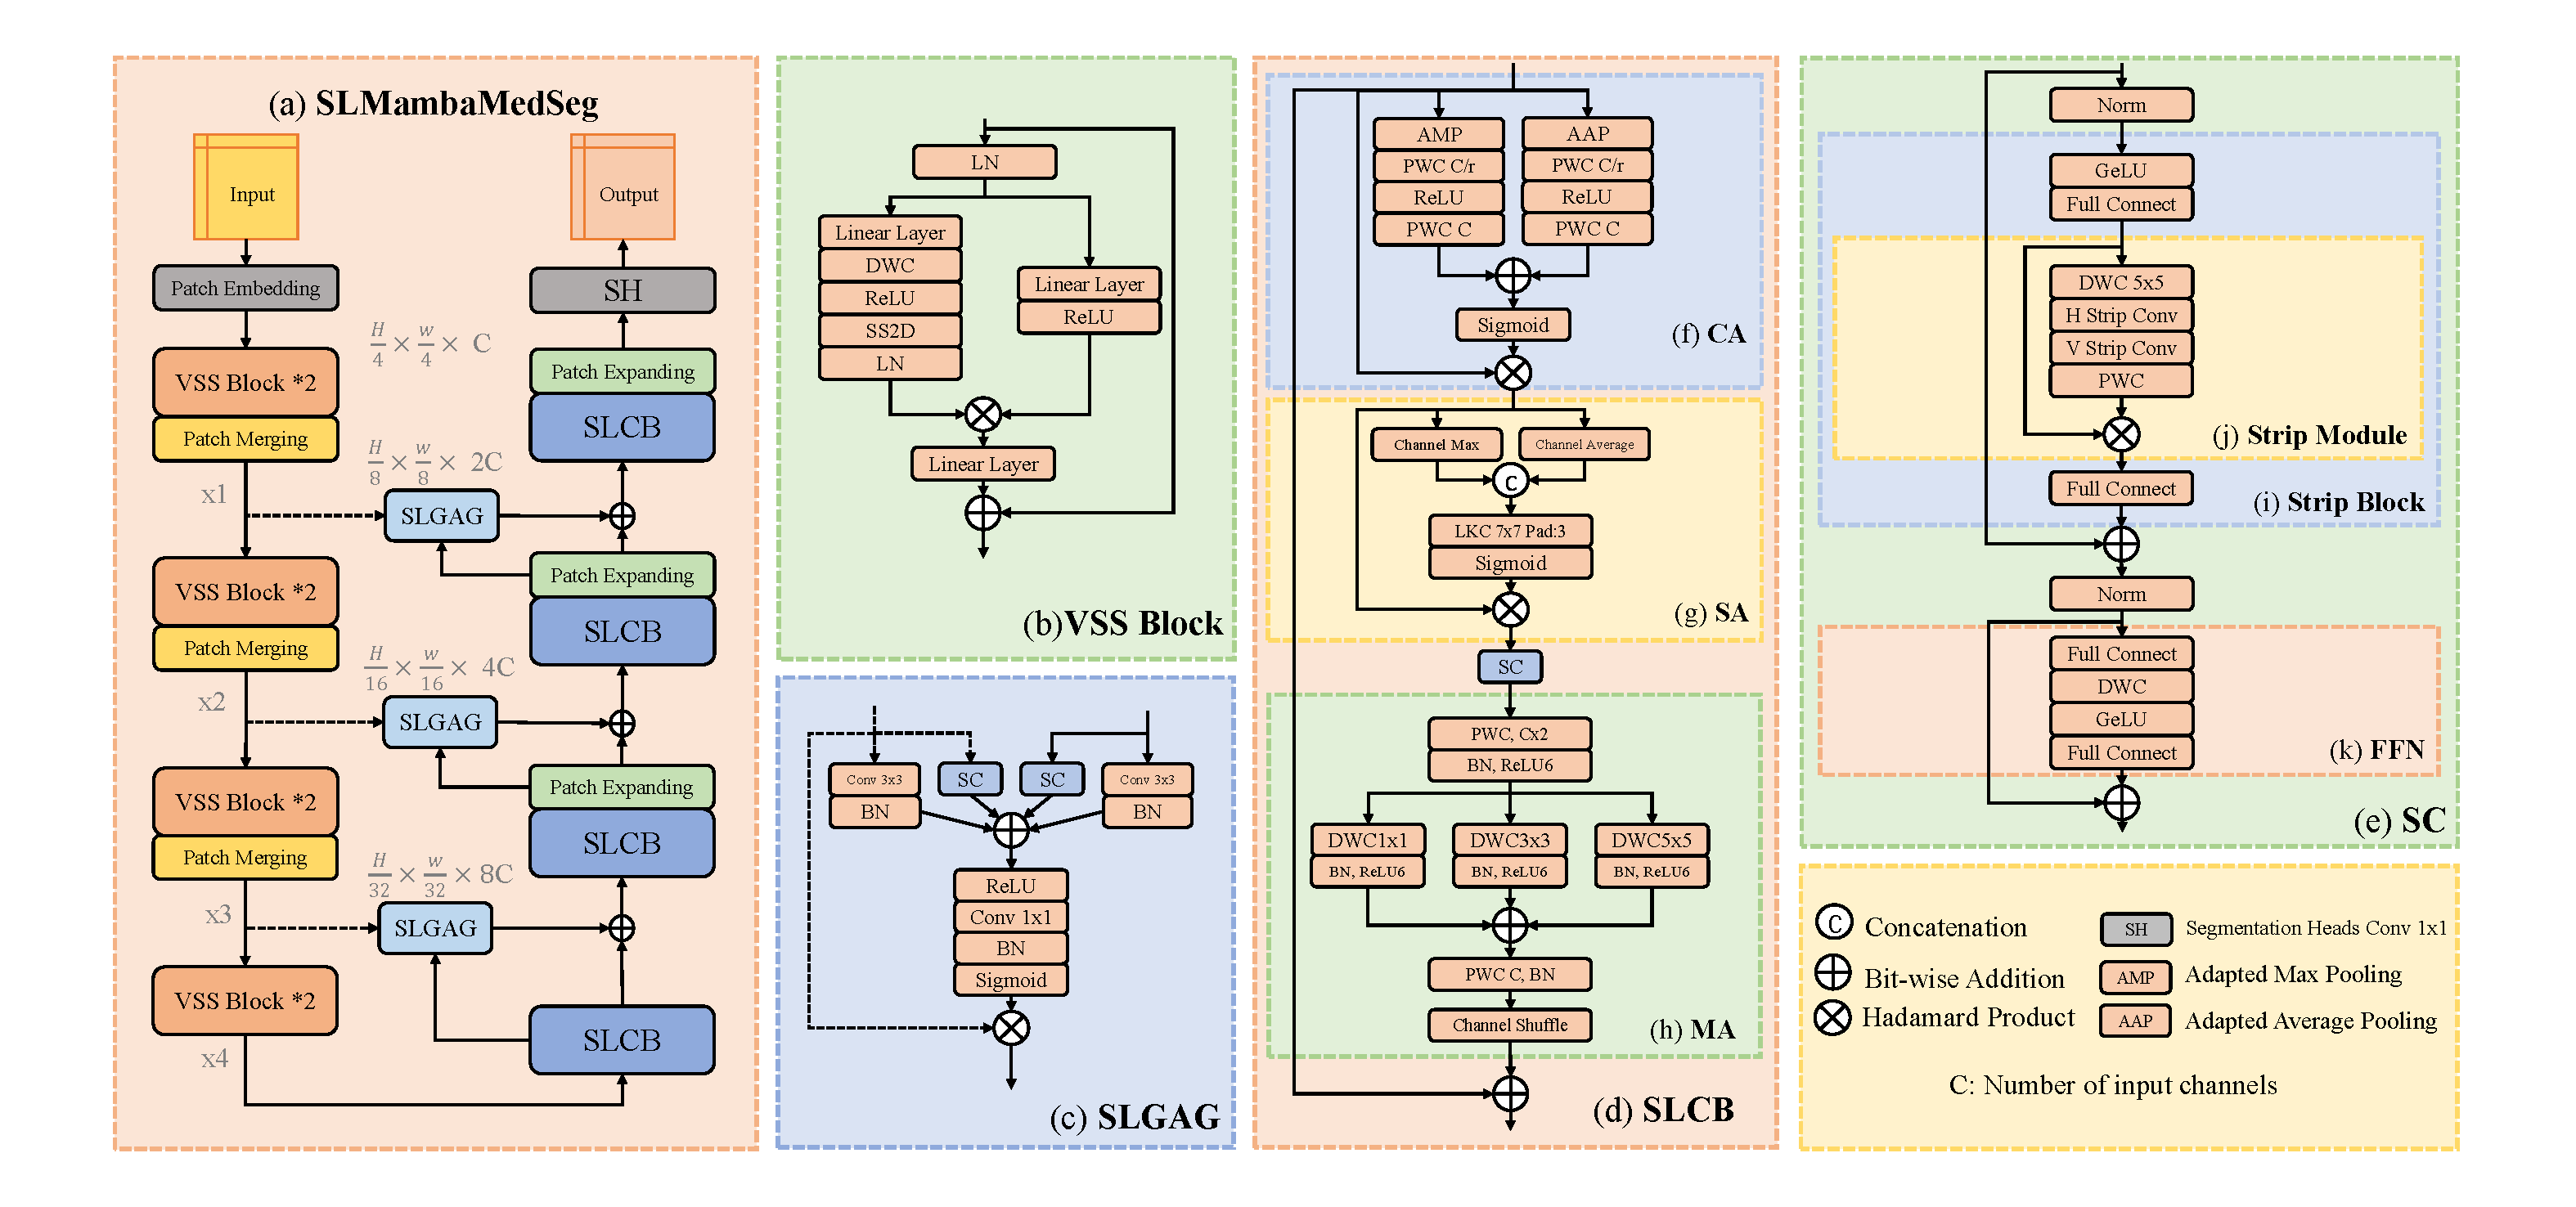
\includegraphics[width=\linewidth]{../Figures/SLMambaMedseg.pdf}
\caption{
	(a) The overall architecture of SLMambaMedseg. 
	(b) VSS Block is the main construction of our encoder. 
	(c) Strip Large-kernel grouped attention gate(SLGAG) can enhance features from skip connections.
	(d) Multi-scale Strip Large-kernel convolutional block(SLCB), progressing patches in all dimensions to further enhance features, is the main component of our decoder.
	(e) Strip convolutional block(SC). 
	(f) Channel attention block(CA). 
	(g) Spatial attention block(SA).  
	(h) Multi-scale attention block(MA). 
	(i) Strip block.
	(j)	Strip module.
	(k) Feed-Forward Network(FFN). 
} \label{figure1}
\end{figure*}





\section{Methodology}

This section first introduces the overall architecture of SLMambaMedseg, followed by detailed descriptions of each constituent module.

\subsection{SLMambaMedseg}

Figure \textcolor{red}{\ref{figure1}} (a) presents the overall architecture of SLMambaMedseg, which follows the U-shaped encoder-decoder design \cite{ronneberger2015unet}. Specifically, SLMambaMedseg comprises a Patch Embedding layer for initial tokenization, four-stage VSS Blocks \cite{liu2024vmamba,gu2023mamba} as the encoder, four-stage SLCBs as the decoder, a Segmentation Head (SH) layer for final projection, and SLGAGs as skip connections.

In the Patch Embedding layer, the input image $x \in \mathbb{R}^{H\times W\times 3}$ is partitioned into non-overlapping $4 \times 4$ patches, producing $x' \in \mathbb{R}^{\frac{H}{4} \times \frac{W}{4} \times C}$ via linear projection to dimension $C$. Before entering the encoder, $x'$ is normalized via layer normalization.

For the encoder, eight VSS Blocks are distributed across four stages, with each stage comprising two VSS Blocks. A patch merging operation is applied at the end of the first three stages to downsample the spatial dimensions of the input features while simultaneously doubling the channel capacity \cite{liu2021swin}. Consequently, the channel counts for the four stages are denoted as $[C, 2C, 4C, 8C]$.

For the decoder, four Multi-scale Strip Large-kernel Convolutional Blocks (SLCBs) progressively refine the hierarchical pyramid features extracted from the encoder via skip connections (i.e., $x_1$, $x_2$, $x_3$, and $x_4$, as illustrated in Figure \ref{figure1}) \cite{lin2017feature}. A patch expanding operation is employed following each of the first three SLCBs to progressively restore the spatial resolution \cite{cao2023swin}. The channel counts for the decoder stages follow the reverse order: $[8C, 4C, 2C, C]$.

To bridge the semantic gap between the encoder and decoder, three Strip Large-Kernel Grouped Attention Gates (SLGAGs) are integrated within the skip connections \cite{oktay2018attention}. The features that are upsampled in the patch expanding layer are subsequently element-wise added to the refined outputs from the corresponding SLGAGs.

Finally, a Segmentation Head (SH) layer is applied to project the fused features and produce the final segmentation output.

\subsection{VSS Block}

As depicted in Figure \textcolor{red}{\ref{figure1}} (b), the VSS Block, derived from VMamba \cite{zhu2024vim,liu2024vmamba}, serves as the core module of our encoder. The input patches $x$ are first layer-normalized and then split into two parallel branches: one branch performs global context modeling, while the other preserves local features.

The global branch processes the input through a linear layer $LL(\cdot)$, a depthwise separable convolution $DWC(\cdot)$, and an activation function $R(\cdot)$. The resulting features are then fed into $SS2D(\cdot)$ for selective scan-based feature extraction, followed by layer normalization $LN(\cdot)$. The local branch applies only a linear layer $LL(\cdot)$ and an activation function $R(\cdot)$, retaining fine-grained spatial details.

The outputs from both branches are merged via a Hadamard product after each passes through an additional linear layer $LL(\cdot)$. Finally, the merged features are added to the initial input $x$ via a residual connection.

The $VSS(.)$ can be formulated as in Equation \textcolor{red}{1}:
\begin{scriptsize} 
\begin{align} 
  VSS(x) = x + SS2D\left(\text{LN}\left(\text{DWC}\left(\text{LL}(x)\right)\right)\right) \otimes \sigma\left(\text{LL}(x)\right)
\end{align} 
\end{scriptsize}



\subsection{Strip Large-kernel Grouped Attention Gate (SLGAG)}

We introduce the Strip Large-kernel Grouped Attention Gate (SLGAG) to enhance the activation of relevant features while suppressing irrelevant ones.

As shown in Figure \textcolor{red}{\ref{figure1}} (c), SLGAG accepts two inputs: $g$ from a patch expanding layer in the decoder, and $x$ from the corresponding encoder stage via skip connection. Both inputs share identical spatial dimensions to enable valid element-wise operations. Each input is processed by a $3 \times 3$ convolution ($Cnv_{3\times 3}(\cdot)$) and a strip convolution ($SC(\cdot)$) in parallel. The resulting feature maps are batch-normalized ($BN(\cdot)$) and merged via element-wise addition. The combined feature map is activated by a ReLU function $R(\cdot)$, then passed through a $1 \times 1$ convolution ($Cnv_{1\times 1}(\cdot)$) to produce a single-channel attention map. This attention map is subsequently normalized by $BN(\cdot)$ and passed through a sigmoid activation $\sigma(\cdot)$ to yield the attention coefficients.

Finally, the initial skip-connection features $x$ are element-wise multiplied by the attention coefficients to produce the gated output.

The $SLGAG(.)$ can be formulated as in Equation \textcolor{red}{2}: 
\begin{scriptsize}
\begin{align}
	SLGAG(g,x) = x \otimes \sigma(BN(Cnv_{1\times 1}(R(SC(g) + BN(Cnv_{3\times 3}(g)) + SC(x) + BN(Cnv_{3\times 3}(x))))))
\end{align}
\end{scriptsize}

\subsection{Multi-scale Strip Large-kernel Convolutional Block (SLCB)}

We introduce the Multi-scale Strip Large-kernel Convolutional Block (SLCB) as the core building block of our decoder, as depicted in Figure \textcolor{red}{\ref{figure1}} (d). The SLCB comprises four sub-modules arranged sequentially: a Channel Attention block (CA) that identifies the most relevant channels, a Spatial Attention block (SA) that highlights the most informative spatial regions, a Strip Convolution block (SC) that enhances feature extraction for thin and elongated structures, and a Multi-scale Attention block (MA) that enriches contextual relationships across multiple receptive fields.

\textbf{Channel Attention Block (CA)}\cite{woo2018cbam}: As depicted in Figure \textcolor{red}{\ref{figure1}} (f), the input $x$ first enters the CA module and is split into two parallel branches. In each branch, $x$ undergoes adaptive max pooling ($AMP(\cdot)$) and adaptive average pooling ($AAP(\cdot)$), respectively \cite{he2014spatial}, to extract the most salient per-channel statistics from the entire feature map. For each pooled descriptor, two point-wise convolution blocks \cite{lin2013network} are applied: $PWC_{C/r}(\cdot)$ (with reduction ratio $r=16$) to compress the channel dimension, and $PWC_C(\cdot)$ to restore it, with an activation function $R(\cdot)$ placed between them. The two resulting feature vectors are combined via element-wise addition and passed through a sigmoid activation $\sigma(\cdot)$. Finally, the resulting channel attention weights are element-wise multiplied with the initial input $x$.

The $CA(.)$ can be formulated as in Equation \textcolor{red}{3}:
\begin{scriptsize}   
\begin{align}
  CA(x) = x \otimes \sigma(PWC_{C}(R(PWC_{C/r}((AMP(x))))) + PWC_{C}(R(PWC_{C/r}(AAP(x)))))
\end{align}
\end{scriptsize}

\textbf{Spatial Attention Block (SA)}\cite{woo2018cbam}: As depicted in Figure \textcolor{red}{\ref{figure1}} (g), following a design analogous to the CA module, the input $x$ is first processed along the channel dimension: max pooling ($CH_{max}(\cdot)$) and average pooling ($CH_{average}(\cdot)$) are applied to aggregate spatial information into two 2D descriptors. These descriptors are concatenated and then fed into a large-kernel convolution $LKC(\cdot)$ with a $7 \times 7$ kernel (padding = 3) to capture local spatial context. The resulting feature map is passed through a sigmoid activation $\sigma(\cdot)$ and element-wise multiplied with the initial input $x$.

The $SA(.)$ can be formulated as in Equation \textcolor{red}{4}:
\begin{scriptsize}
\begin{align}
  SA(x) = x \otimes \sigma(LKC([CH_{max}(x); CH_{average}(x)]))
\end{align}
\end{scriptsize}

\textbf{Multi-scale Attention Block (MA)}: As depicted in Figure \textcolor{red}{\ref{figure1}} (h), the input $x$ first undergoes channel expansion via a point-wise convolution $PWC_{C\times 2}(\cdot)$ (expansion factor of 2), followed by batch normalization $BN(\cdot)$ and a ReLU6 activation $R6(\cdot)$ \cite{howard2017mobilenets}. The expanded features are then processed in parallel by three depthwise separable convolution layers ($DWC(\cdot)$) with different kernel sizes to capture multi-scale context (the number and size of kernels are configurable). The outputs from the three branches are summed, and a channel shuffle operation $CSF(\cdot)$ \cite{zhang2018shufflenet} is applied to enhance cross-channel information flow. The shuffled features are then projected back to the original channel dimension via a point-wise convolution $PWC_C(\cdot)$, followed by batch normalization $BN(\cdot)$. Finally, the result is added to the initial input $x$ via a residual connection.

The $MA(.)$ can be formulated as in Equation \textcolor{red}{5}:
\begin{scriptsize}   
\begin{align}
  MA(x)=x+BN(PWC_{C}(CSF(\sum_{}^{}DWC_{k_i}(R6(BN(PWC_{C\times2}(x)))))))
\end{align}
\end{scriptsize}



% Synapse 可视化 %
\begin{figure*}[h]
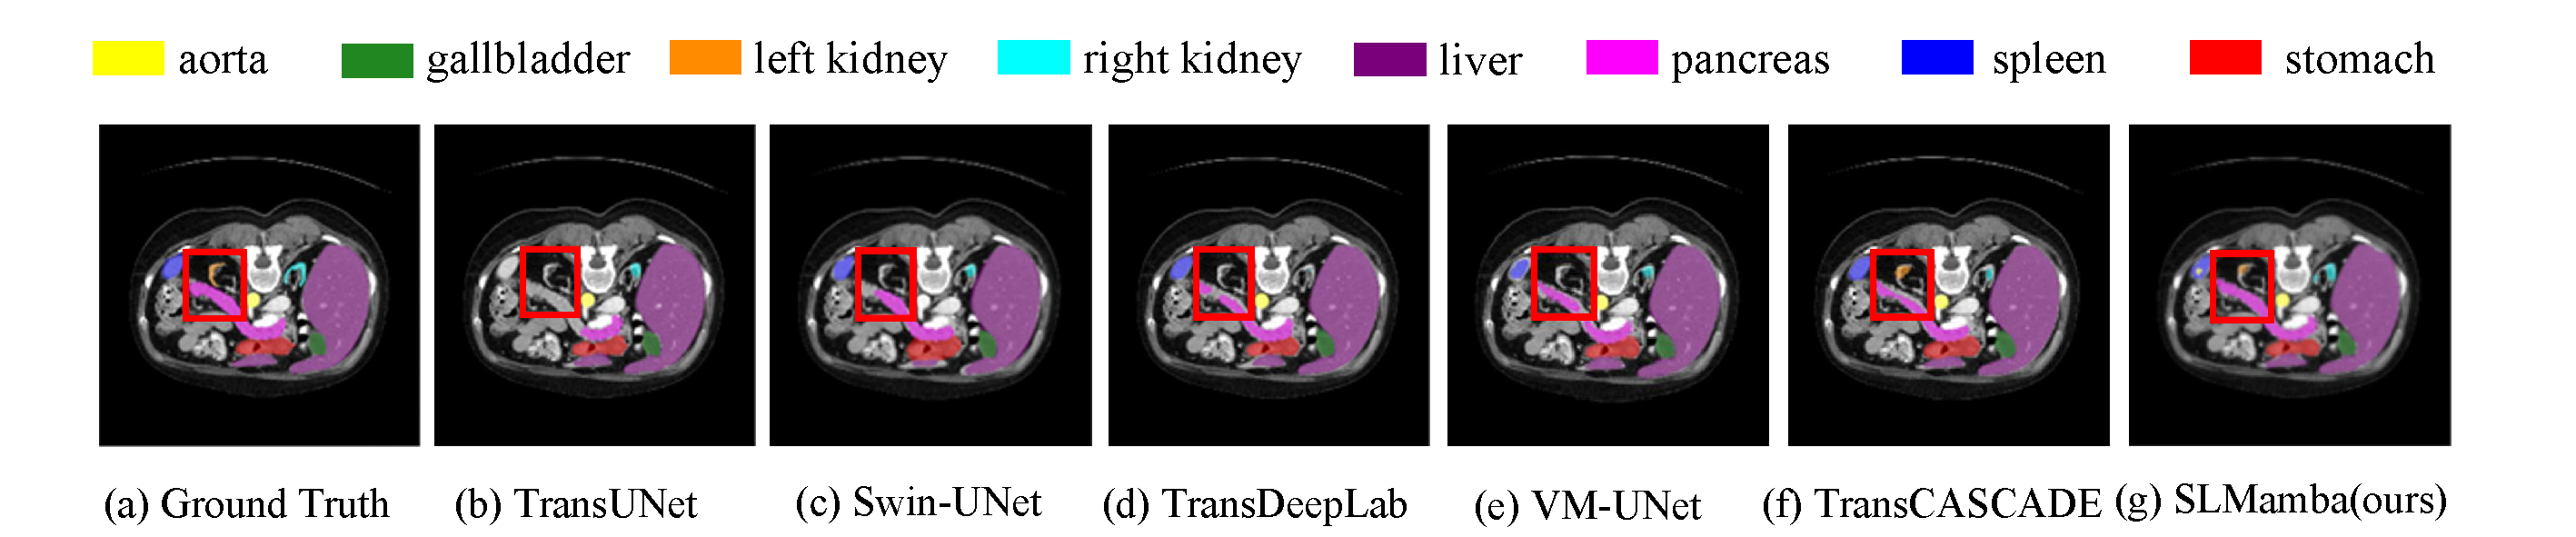
\includegraphics[width=\linewidth]{../Figures/Synapse.pdf}
\caption{
	Qualitative results on Synapse datasets are shown. The red rectangular box highlights incorrectly segmented structures by SOTA methods.
} \label{figure2}
\end{figure*}

% Synapse 结果 %
\begin{table*}[h]
\footnotesize
\centering
\label{f1}
\begin{tabular}{l|cc|cccccccc}\hline
Methods & DICE$\uparrow$ & HD95$\downarrow$ &Aor.& Gal. &Kid.(L) &Kid.(R) &Liv. &Pan. &Spl. &Sto. \\\hline

nnU-Net\cite{isensee2021nnu} & [TODO] & [TODO] & [TODO] & [TODO] & [TODO] & [TODO] & [TODO] & [TODO] & [TODO] & [TODO] \\
UNet\cite{ronneberger2015unet} & 70.11& 44.69& 84.00 &56.70& 72.41& 62.64& 86.98& 48.73& 81.48& 67.96 \\
AttnUNet\cite{oktay2018attention}& 71.70& 34.47& 82.61& 61.94& 76.07& 70.42& 87.54& 46.70& 80.67& 67.66 \\
TransUNet\cite{chen2021transunet} & 77.48 &31.69& 87.23 &63.13 &81.87 &77.02 &94.08 &55.86& 85.08& 75.62	\\
SSFormer\cite{wang2022stepwise}& 78.01& 25.72&  82.78& 63.74& 80.72& 78.11& 93.53& 61.53& 87.07& 76.61 \\
PolypPVT\cite{dong2021polyp} & 78.08& 25.61&  82.34& 66.14& 81.21& 73.78& 94.37& 59.34& 88.05& 79.4 \\
Swin-UNet\cite{cao2021swinunet} & 79.56 & 21.55 & 85.47 &66.53 &83.28 &79.61& 94.29 &56.58& 90.66& 76.60	\\
MT-UNet\cite{wang2022mixed} & 78.59 &26.59& 87.92& 64.99& 81.47& 77.29& 93.06& 59.46& 87.75& 76.81\\
MEW-UNet\cite{ruan2022mew} & 78.92& 16.44& 86.68& 65.32& 82.87& 80.02& 93.63& 58.36& 90.19& 74.26\\
PVT-CASCADE\cite{rahman2023medical} & 81.06& 20.23& 83.01& 70.59& 82.23& 80.37& 94.08& 64.43& 90.1& 83.69 \\
TransDeepLab\cite{azad2022transdeeplab} & 80.16& 21.25& 86.04& 69.16& 84.08& 79.88& 93.53& 61.19& 89.00& 78.40\\
VM-UNet\cite{ruan2024vmunet} & 81.08& 19.21& 86.40& 69.41& 86.16& 82.76& 94.17& 58.80& 89.51& 81.40 \\
TransCASCADE\cite{rahman2023transcascade} & 82.68 &17.34 & 86.63 &68.48& 87.66& 84.56& \textbf{94.43}& \textbf{65.33}& 90.79& 83.52\\
\hline
SLMambaMedseg(ours) & \textbf{83.36}& \textbf{16.18}& \textbf{88.43}& \textbf{70.94}& \textbf{88.57}& \textbf{84.79}& 94.33& 64.59& \textbf{91.23}& \textbf{84.01} \\\hline
\end{tabular}
\caption{Results on Synapse Multi-Organ Segmentation. DICE scores are reported for individual organs. $\uparrow$ denotes higher the better, $\downarrow$ denotes lower the better. The best results are in bold.}
\label{table1}
\end{table*}




\subsection{Strip Convolution Block (SC)}

The Strip Convolution Block (SC) \cite{hou2020strip,liu2023slak,chu2021active} is integrated into SLMambaMedseg to address the limitations of traditional square-kernel convolutions in capturing elongated and curvilinear anatomical structures.

The SC module is illustrated in Figure \textcolor{red}{\ref{figure1}} (e). The input $x$ first passes through layer normalization, a fully connected layer, and a GELU activation function \cite{hendrycks2016gelu}. The normalized features $x'$ then enter the Strip Module, the core component of SC, as depicted in Figure \textcolor{red}{\ref{figure1}} (j).

Within the Strip Module, a large-kernel depthwise convolution ($5 \times 5$) first extracts local contextual features. Subsequently, two sequential depthwise strip convolutions with kernel sizes $1 \times N$ and $N \times 1$ are applied to capture objects of high aspect ratios, followed by a point-wise convolution for channel mixing.

The output of the Strip Module, denoted as $Z$, undergoes a Hadamard product with $x'$ to produce $Z'$, which is then element-wise added to a fully-connected projection of $x$. This intermediate result is added to $x$ once more, yielding $Y$. Finally, $Y$ is normalized and processed by a feed-forward network (FFN), with the FFN output added to the normalized $Y$ via a residual connection to produce the final output $SC(x)$.


\subsection{Loss Function}
\label{sec:loss}

To optimize the SLMambaMedseg for high-precision medical image segmentation, we employ a hybrid loss function, denoted as $L_{total}$, which synergistically combines Soft Dice Loss and Focal Loss.

The rationale behind this design is two-fold. First, Soft Dice Loss is utilized to maximize the spatial overlap between the segmented masks and the ground truth, effectively mitigating the issues caused by the severe class imbalance inherent in medical datasets (e.g., small lesion areas versus large background regions). Second, to address the challenge of hard-to-classify pixels near anatomical boundaries, Focal Loss is integrated. By introducing a modulating factor $(1 - p_t)^\gamma$, Focal Loss reshapes the standard cross-entropy loss to down-weight easy examples and focus the model's learning capacity on ambiguous regions and sparse foreground pixels.

The objective function is formulated as in Equation \textcolor{red}{6}:

\begin{footnotesize}   
\begin{align}
  L_{total} = \lambda_{dice} L_{Dice} + \lambda_{focal} L_{Focal}
\end{align}
\end{footnotesize}

where $\lambda_{dice}$ and $\lambda_{focal}$ are hyper-parameters representing the weighting coefficients for each component. In our experiments, we empirically set $\lambda_{dice} = 1$ and $\lambda_{focal} = 1$ to maintain a balanced gradient flow throughout the backpropagation process, ensuring both global structural consistency and local boundary sharpness.

\section{Experiments}

This section will present the details of implementation followed by a comparative analysis of our SLMambaMedseg against SOTA methods, including the performance of the complete model on the datasets and the details of the ablation study.

\subsection{Implementation details}

To evaluate the proposed SLMambaMedseg, comprehensive experiments are conducted on two widely adopted public benchmarks: the Synapse multi-organ segmentation dataset \cite{landman2015miccai} and the Automated Cardiac Diagnosis Challenge (ACDC) dataset \cite{bernard2018deep}.

\textbf{Datasets.} The Synapse dataset comprises 30 abdominal CT scans with 13 abdominal organs annotated. Following the standard protocol \cite{chen2021transunet,cao2021swinunet}, we adopt the official split of 18 training cases and 12 testing cases. The ACDC dataset contains 100 cardiac MRI scans from 100 patients, each with annotations for the right ventricle (RV), left ventricle (LV), and myocardium (Myo). We follow the standard split of 70 training cases, 10 validation cases, and 20 testing cases \cite{bernard2018deep}. Patient-level separation is strictly enforced to prevent data leakage between training and test sets.

\textbf{Preprocessing.} All images are uniformly resized to a spatial resolution of $224 \times 224$, and intensity values are normalized to zero mean and unit variance. To mitigate the risk of overfitting and enhance generalization, standard data augmentation techniques including random flipping and random rotation are employed.

\textbf{Training Protocol.} We set the batch size to 32 and employ the AdamW optimizer \cite{loshchilov2017decoupled} with an initial learning rate of $1 \times 10^{-5}$ and weight decay of $1 \times 10^{-3}$. A cosine annealing learning rate scheduler \cite{loshchilov2016sgdr} is applied with a maximum of 50 iterations and a minimum learning rate of $1 \times 10^{-5}$. The entire training process spans 300 epochs. The random seed is set to 42. For the hybrid loss function, the Focal Loss parameters are set to $\alpha = 0.5$ and $\gamma = 0.5$, and the Dice Loss uses a smoothing factor of $\epsilon = 1 \times 10^{-3}$.

\textbf{Evaluation.} For quantitative assessment, two primary metrics are used: the Dice Similarity Coefficient (DSC) to measure region-based overlap \cite{milletari2016v}, and the 95\% Hausdorff Distance (HD95) to evaluate boundary-based accuracy \cite{huttenlocher1993comparing}. All reported results are averaged over 5 independent runs with different random seeds, and standard deviations are reported alongside the mean scores. Statistical significance is assessed using [TODO: statistical\_test, e.g., paired t-test].

All experiments are implemented using the PyTorch framework and executed on a single NVIDIA RTX 5090 GPU.










\subsection{Experimental Results}

We compare SLMambaMedseg against state-of-the-art models spanning diverse architectural paradigms on both Synapse and ACDC datasets. The baselines include pure CNN models (UNet\cite{ronneberger2015unet}), pure Transformer models (Swin-UNet\cite{cao2021swinunet,cao2023swin}), pure Mamba models (VM-UNet\cite{ruan2024vmunet}), CNN-Transformer hybrid models (TransUNet\cite{chen2021transunet}, TransCASCADE\cite{rahman2023transcascade}), and other recent SOTA methods. For fair comparison, all baseline results are reproduced under our experimental setting unless otherwise noted. The results demonstrate that SLMambaMedseg consistently achieves the best performance across both datasets.



\subsubsection{Results on Synapse Multi-Organ Segmentation}

Results on Synapse are presented in Table \textcolor{red}{\ref{table1}}. Among the compared methods, SLMambaMedseg achieves the best overall performance with a mean DSC of 83.36\% and a mean HD95 of 16.18 mm, outperforming TransCASCADE\cite{rahman2023transcascade} (82.68\% / 17.34 mm) and VM-UNet\cite{ruan2024vmunet} (81.08\% / 19.21 mm). Two factors contribute to this improvement. First, the Vision Mamba encoder provides efficient global context modeling with linear complexity. Second, and more critically, the SLCB decoder with strip and large-kernel convolutions provides stronger local feature refinement than the VSS-block-based decoder used in pure Mamba architectures such as VM-UNet. Notably, SLMambaMedseg achieves the highest per-organ DSC in six out of eight organ categories, with particularly strong gains on the left kidney (88.57\%) and stomach (84.01\%).

Figure \textcolor{red}{\ref{figure2}} presents qualitative comparisons on the Synapse dataset. Several baseline models exhibit notable segmentation failures: TransUNet\cite{chen2021transunet}, Swin-UNet\cite{cao2021swinunet}, TransDeepLab\cite{azad2022transdeeplab}, and VM-UNet\cite{ruan2024vmunet} all fail to adequately segment the left kidney. Additionally, TransUNet and Swin-UNet miss a substantial portion of the pancreas, and TransDeepLab shows similar but less severe limitations. In contrast, SLMambaMedseg produces segmentation masks that more faithfully delineate the ground truth, particularly for small and slender organs such as the kidneys and pancreas.




\subsubsection{Results of ACDC Segmentation}

Results on ACDC are presented in Table \textcolor{red}{\ref{table2}}. SLMambaMedseg achieves the best overall performance with a mean DSC of 93.51\%, surpassing TransCASCADE\cite{rahman2023transcascade} (92.12\%) and VM-UNet\cite{ruan2024vmunet} (91.63\%). The model also attains the highest per-structure DSC for all three cardiac structures: RV (92.22\%), Myo (90.58\%), and LV (97.23\%). These results demonstrate that replacing the VSS-based decoder with an enhanced convolutional decoder yields consistent gains, particularly for structures with complex boundaries such as the myocardium.

Figure \textcolor{red}{\ref{figure3}} presents qualitative comparisons on the ACDC dataset. Swin-UNet\cite{cao2021swinunet} incorrectly omits the middle portion of the left ventricle, while TransUNet\cite{chen2021transunet} misses the left portion of the myocardium. TransDeepLab\cite{azad2022transdeeplab} fails to capture the full myocardium and introduces false-positive predictions for the left ventricle. Although VM-UNet\cite{ruan2024vmunet} and TransCASCADE\cite{rahman2023transcascade} produce approximately correct segmentations, their boundary delineation is less smooth and precise compared to SLMambaMedseg, which yields the most anatomically faithful contours.


% ACDC可视化 %
\begin{figure*}[h]
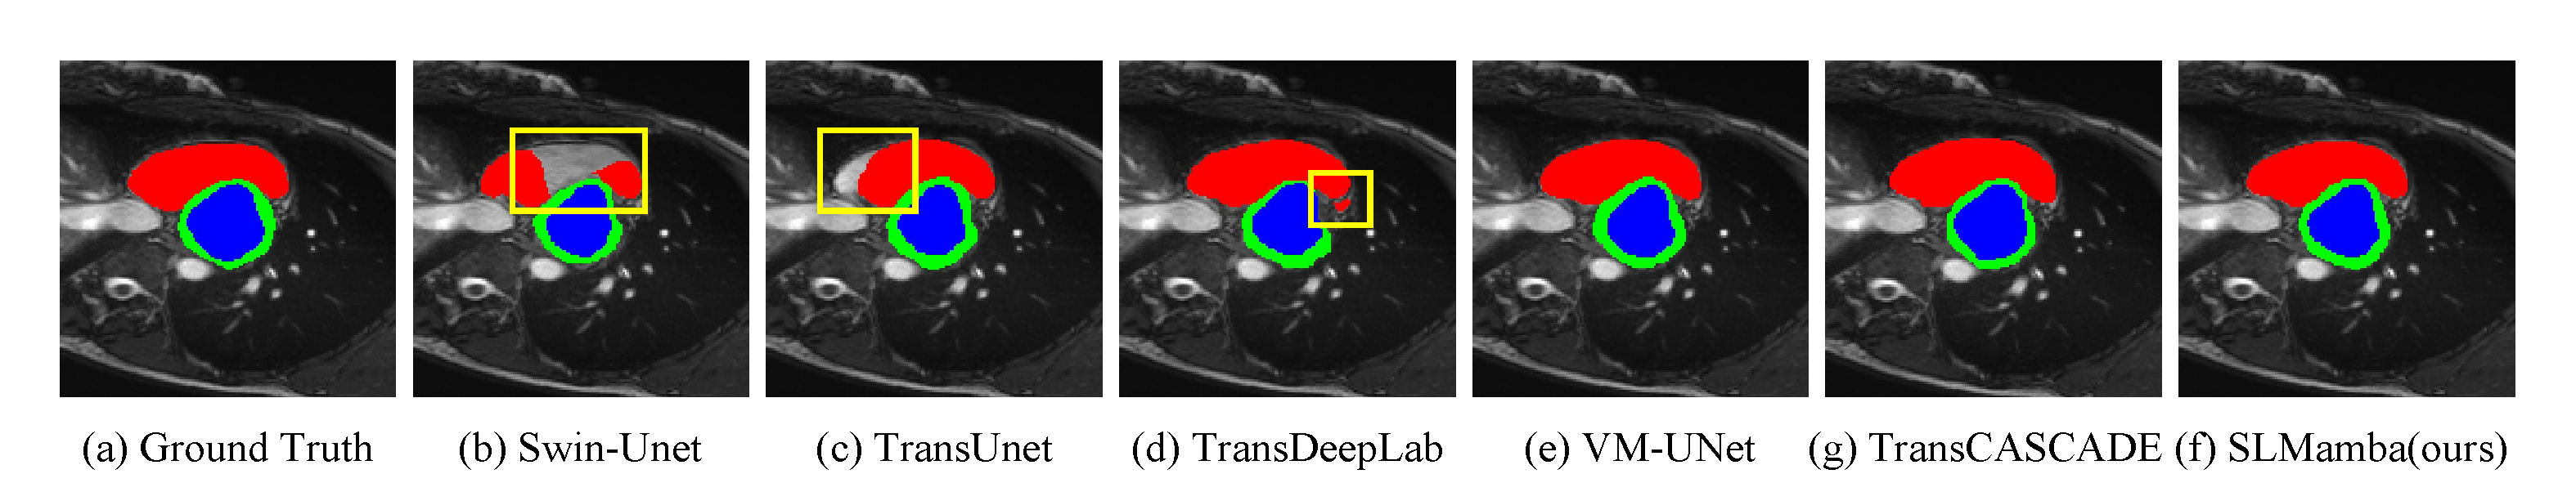
\includegraphics[width=\linewidth]{../Figures/ACDC.pdf}
\caption{
	Qualitative results on ACDC datasets are shown. Red represents the right ventricle, blue represents the left ventricle, and green represents the myocardium. The yellow rectangular box highlights incorrectly segmented regions by SOTA methods.
} \label{figure3}
\end{figure*}


% ACDC 结果 %
\begin{table}[h]
\footnotesize
\centering
\begin{tabular}{l|c|ccc}\hline
Methods & DICE$\uparrow$  &RV &Myo& LV\\\hline
nnU-Net\cite{isensee2021nnu} & [TODO] & [TODO] & [TODO] & [TODO] \\
TransUNet\cite{chen2021transunet} & 89.71& 86.67& 87.27& 95.18 \\
SwinUNet\cite{cao2021swinunet} & 90.00& 88.55& 85.62& 95.83 \\
HiFormer\cite{heidari2023hiformer} & 90.12& 91.06& 84.54& 94.77 \\
TransDeepLab\cite{azad2022transdeeplab} & 90.41& 91.45& 84.54& 95.23 \\
MT-UNet\cite{wang2022mixed} & 90.43& 86.64& 89.04& 95.62 \\
MISSFormer\cite{huang2022missformer} & 90.86& 89.55& 88.04& 94.99 \\
ParaTransCNN\cite{sun2024paratranscnn} & 91.31& 92.76& 85.84& 95.34 \\
VM-UNet\cite{ruan2024vmunet} & 91.63& 90.25& 89.14& 95.50 \\
TransCASCADE\cite{rahman2023transcascade} & 92.12& 90.65& 89.68& 96.02 \\
\hline
SLMambaMedseg(ours) & \textbf{93.51} & \textbf{92.22} & \textbf{90.58} &\textbf{97.23} \\\hline
\end{tabular}
\caption{ Results on ACDC. DICE scores($\%$)are reported for individual organs.$\uparrow$ denotes higher the better. The best results are in bold.}
\label{table2}
\end{table}



% 效率对比 %
\begin{table}[h]
\footnotesize
\centering
\begin{tabular}{l|ccccc}\hline
Methods & Params (M)$\downarrow$ & FLOPs (G)$\downarrow$ & Inference (ms)$\downarrow$ & GPU Mem. (GB)$\downarrow$ & Train Time (h)$\downarrow$ \\\hline
UNet\cite{ronneberger2015unet} & 34.53M & 65.53G & [TODO] & [TODO] & [TODO] \\
Swin-UNet\cite{cao2021swinunet} & 27.17M & 5.95G & [TODO] & 0.31 GB & [TODO] \\
TransUNet\cite{chen2021transunet} & 105.28M & 593.00G & [TODO] & 7.55 GB & [TODO] \\
VM-UNet\cite{ruan2024vmunet} & 27.43M & 3.15G & [TODO] & 0.42 GB & [TODO] \\
TransCASCADE\cite{rahman2023transcascade} & 35.12M & 8.29G & [TODO] & [TODO] & [TODO] \\
\hline
SLMambaMedseg(ours) & 17.20M & 2.63G & [TODO] & 3.38GB & [TODO] \\\hline
\end{tabular}
\caption{Computational efficiency comparison. Params: number of parameters; FLOPs: floating-point operations per input (measured at $224\times 224$); Inference: average inference time per image; GPU Mem.: peak GPU memory during inference; Train Time: total training time on Synapse. $\downarrow$ denotes lower is better.}
\label{table_efficiency}
\end{table}

% 编码器消融实验 %
\begin{table}[h]
\small
\centering
\begin{tabular}{l|cc|c}\hline
\multirow{2}{*}{Methods} & \multicolumn{2}{c|}{Synapse} & ACDC \\\cline{2-4}
& DICE$\uparrow$ & HD95$\downarrow$ & DICE$\uparrow$ \\\hline
SLCNNMedseg & 81.93 &18.27& 89.94\\
SLTransMedseg & 82.76 & 16.62 & 91.05\\\hline
SLMambaMedseg & \textbf{83.36} & \textbf{16.18} & \textbf{93.51} \\\hline
\end{tabular}
\caption{Results of how different encoders affect performance of segmentaion on Synapse and ACDC datasets. $\uparrow$ denotes higher the better, $\downarrow$ denotes lower the better. The best results are in bold.}
\label{table3}
\end{table}

\subsection{Ablation Studies}

%\subsubsection{Structure Ablation}

\subsubsection{Effect of Mamba Encoder}

To evaluate the effect of different encoder architectures, we construct two variants of SLMambaMedseg by replacing the VSS encoder with a pure CNN encoder (as in UNet \cite{ronneberger2015unet}) and a pure Transformer encoder (as in Swin-UNet \cite{cao2021swinunet}), denoted as SLCNNMedseg and SLTransMedseg, respectively. Table \textcolor{red}{\ref{table3}} reports the results on both Synapse and ACDC datasets. SLMambaMedseg with the Vision Mamba encoder consistently outperforms both alternatives, achieving 83.36\% DSC on Synapse compared to 82.76\% (SLTransMedseg) and 81.93\% (SLCNNMedseg). This trend holds on ACDC as well. We attribute the advantage of the Mamba encoder to its ability to model long-range dependencies with linear complexity, which enables more effective global context aggregation without the quadratic overhead of self-attention.


% SLGAG 消融实验 %
\begin{table}[h]
\footnotesize
\centering
\begin{tabular}{l|ccc|c}\hline
\multirow{2}{*}{Methods} & \multicolumn{3}{c|}{Synapse} & ACDC \\\cline{2-5}
& DICE$\uparrow$ & HD95$\downarrow$ &Kid.(L) & DICE$\uparrow$ \\\hline
SLMambaMedseg W/o SLGAG & 81.80 & 18.47 &83.97  & 90.79\\\hline
SLMambaMedseg & \textbf{83.36} & \textbf{16.18} &\textbf{88.57}  & \textbf{93.51} \\\hline
\end{tabular}
\caption{Results of Ablation Experiment of how Strip Large-kernel Group Attention Gate(SLGAG) affects on Synapse and ACDC datasets. $\uparrow$ denotes higher the better, $\downarrow$ denotes lower the better.}
\label{table4}
\end{table}

% MA 卷积核策略 消融实验%
\begin{table*}[h]
\small
\centering
\begin{tabular}{l|cccccccccc}\hline
\multirow{2}{*}{Methods} & \multicolumn{10}{c}{Kernel Strategies} \\\cline{2-11}
& [1] & [3] & [5] & [1,3] & [3,5] & [3,3,3] &[1,3,5]& [5,5,5] &[3,5,7] &[1,3,5,7]  \\\hline
Synapse& 83.11& 82.93& 82.64& 83.02& 83.25& 82.73 & \textbf{83.36}& 82.98& 83.15& 83.20 \\
ACDC & 91.14 &91.94 & 91.89 &92.28& 91.93& 92.35& \textbf{93.51}& 92.32& 92.12& 92.43\\
\hline
\end{tabular}
\caption{Results of different depthwise convolution kernel strategies effect on Synapse and ACDC. In $[k_{1},k_{2},...,k_{n}]$, $k_{i}$ means size of each kernel, $\sum_{1}^{n}k_{i}$ means total number of the kernels. The best results are in bold.}
\label{table5}
\end{table*}


\subsubsection{Effect of SLGAG}

To evaluate the effectiveness of the SLGAG mechanism, we conduct an experiment in which the SLGAG-enhanced skip connections are replaced with standard unprocessed skip connections, and compare this variant against the full SLMambaMedseg on both Synapse and ACDC datasets. The results are reported in Table \textcolor{red}{\ref{table4}}. SLMambaMedseg with SLGAG consistently outperforms the variant without it, with particularly notable gains on small and elongated structures such as the left kidney (88.57\% vs.\ 83.97\% DSC on Synapse). This confirms that the strip convolutions within SLGAG are effective at capturing fine-grained, anisotropic features that standard skip connections fail to preserve.


\subsubsection{Effect of Convolution Kernel Size in MA}

We further investigate the impact of depthwise convolution kernel configurations within the MA module on both Synapse and ACDC datasets. We evaluate ten strategies by varying the number of parallel branches and their kernel sizes, ranging from a single-branch configuration (e.g., $[3]$ or $[5]$) to multi-branch configurations with three or four branches (e.g., $[1,3,5]$ or $[1,3,5,7]$). The results are presented in Table \textcolor{red}{\ref{table5}}. The three-branch configuration $[1,3,5]$ achieves the best performance on both datasets, yielding 83.36\% DSC on Synapse and 93.51\% DSC on ACDC. We attribute this to the complementary nature of the three kernel sizes: the $1 \times 1$ kernel preserves fine local details, the $3 \times 3$ kernel captures mid-range context, and the $5 \times 5$ kernel provides a broader receptive field. Notably, adding more or larger kernels (e.g., $[3,5,7]$ or $[1,3,5,7]$) does not improve performance, suggesting that excessively large kernels may dilute local features and that three branches offer a sufficient diversity of receptive fields.






\subsubsection{Effect of Individual SLCB Components}

To isolate the contribution of each sub-module within the SLCB, we conduct a systematic ablation study by removing one component at a time from the full model. Specifically, we evaluate the following variants: (1) without Channel Attention ($-$CA), (2) without Spatial Attention ($-$SA), (3) without Strip Convolution ($-$SC), and (4) without Multi-scale Attention ($-$MA). All experiments are conducted on the Synapse dataset under identical training settings.

\begin{table}[h]
\footnotesize
\centering
\begin{tabular}{l|cc}\hline
Variant & Synapse DSC$\uparrow$ & HD95$\downarrow$ \\\hline
SLMambaMedseg (full) & 83.36 & 16.18 \\
$-$ CA & 83.14 & 16.42 \\
$-$ SA & 82.95 & 16.65 \\
$-$ SC & 82.78 & 16.89 \\
$-$ MA & 82.54 & 17.13 \\
$-$ All SLCB enhancements & 82.31 & 17.35 \\\hline
\end{tabular}
\caption{Ablation study of individual SLCB components on the Synapse dataset. Each variant removes one component while keeping all others unchanged.}
\label{table_slcb_ablation}
\end{table}

\subsubsection{Effect of Loss Function}

To evaluate the contribution of each loss term, we compare three training configurations on the Synapse dataset: (1) Soft Dice Loss only, (2) Focal Loss only, and (3) the combined Dice + Focal Loss (our default). The weighting coefficients and hyperparameters follow the settings described in Section~\ref{sec:loss}.

\begin{table}[h]
\footnotesize
\centering
\begin{tabular}{l|cc}\hline
Loss Configuration & Synapse DSC$\uparrow$ & HD95$\downarrow$ \\\hline
Dice Loss only & 81.84 & 18.47 \\
Focal Loss only & 82.52 & 17.20 \\
Dice + Focal Loss (ours) & 83.36 & 16.18 \\\hline
\end{tabular}
\caption{Ablation study of loss function configurations on the Synapse dataset.}
\label{table_loss_ablation}
\end{table}

\section{Conclusions}

This paper has presented SLMambaMedseg, a novel medical image segmentation framework that synergizes Vision Mamba-based global encoding with multi-scale strip large-kernel convolutional decoding. By integrating the VSS Block encoder with the proposed SLCB decoder and SLGAG skip connections, the model effectively balances global context modeling with fine-grained local feature extraction, achieving notable improvements in delineating small, elongated, and anatomically intricate structures.

Experimental results on the Synapse and ACDC datasets demonstrate that SLMambaMedseg achieves competitive segmentation accuracy compared to state-of-the-art methods, including VM-UNet and TransCASCADE. Ablation studies validate the effectiveness of the Mamba encoder, the SLGAG mechanism, and the multi-scale kernel strategy within the SLCB module. These findings indicate that the combination of Vision Mamba encoding with strip and large-kernel convolutional decoding is a promising direction for medical image segmentation, and we hope our work encourages further exploration of hybrid architectures that leverage the complementary strengths of state space models and advanced convolutional designs.




\begin{thebibliography}{99}

% 1.1
\bibitem{ronneberger2015unet}
Ronneberger, O., Fischer, P., \& Brox, T. (2015). U-net: Convolutional networks for biomedical image segmentation. In \textit{International Conference on Medical Image Computing and Computer-Assisted Intervention} (pp. 234–241).
\bibitem{milletari2016vnet}
 Milletari, F., Navab, N., \& Ahmadi, S. A. (2016). V-Net: Fully convolutional neural networks for volumetric medical image segmentation. In 2016 fourth international conference on 3D vision (3DV) (pp. 565-571). IEEE. 
\bibitem{isensee2021nnu}
Isensee, F., Jaeger, P. F., Kohl, S. A., Petersen, J., \& Maier-Hein, K. H. (2021). nnU-Net: a self-configuring method for deep learning-based biomedical image segmentation. \textit{Nature Methods}, 18(2), 203–211.


\bibitem{chen2021transunet}
Chen, J., Lu, Y., Yu, Q., Luo, X., Adeli, E., Wang, Y., … \& Zhou, Y. (2021). TransUNet: Transformers make strong encoders for medical image segmentation. \textit{arXiv preprint arXiv:2102.04306}.
\bibitem{cao2021swinunet}
Cao, H., Wang, Y., Chen, J., Jiang, D., Zhang, X., Tian, Q., \& Wang, M. (2021). Swin-Unet: Unet-like pure transformer for medical image segmentation. \textit{arXiv preprint arXiv:2105.05537}.

% 1：2
\bibitem{gu2023mamba}
Gu, A., \& Dao, T. (2023). Mamba: Linear-time sequence modeling with selective state spaces. \textit{arXiv preprint arXiv:2312.00752}.
\bibitem{liu2024vmamba}
Liu, Y., Tian, Y., Zhao, Y., Yu, H., Xie, L., Wang, Y., … \& Ye, Q. (2024). VMamba: Visual State Space Model. \textit{arXiv preprint arXiv:2401.10166}.
\bibitem{zhu2024vim}
Zhu, L., Liao, B., Zhang, Q., Wang, X., Liu, W., \& Wang, X. (2024). Vision Mamba: Efficient visual representation learning with bidirectional state space model. \textit{arXiv preprint arXiv:2401.09417}.
%1.3
\bibitem{ruan2024vmunet}
Ruan, J., \& Xiang, S. (2024). VM-UNet: Vision Mamba UNet for medical image segmentation. \textit{arXiv preprint arXiv:2402.02491}.
\bibitem{ma2024umamba}
Ma, J., Li, F., \& Wang, B. (2024). U-Mamba: Enhancing long-range dependency for biomedical image segmentation. \textit{arXiv preprint arXiv:2401.04722}.
\bibitem{liu2022convnext}
Liu, Z., Mao, H., Wu, C. Y., Feichtenhofer, C., Darrell, T., \& Xie, S. (2022). A convnet for the 2020s. In \textit{Proceedings of the IEEE/CVF conference on computer vision and pattern recognition (pp. 11976-11986)}. 
\bibitem{hou2020strippooling} 
Hou, Q., Zhang, L., Cheng, M. M., \& Feng, J. (2020). Strip pooling: Rethinking spatial pooling for scene parsing. In \textit{Proceedings of the IEEE/CVF conference on computer vision and pattern recognition (pp. 4003-4012)}. 

%====2=====

%2.1

\bibitem{lecun2015deep}LeCun, Y., Bengio, Y., \& Hinton, G. (2015). Deep learning. Nature, 521(7553), 436-444.
\bibitem{he2016resnet}He, K., Zhang, X., Ren, S., \& Sun, J. (2016). Deep residual learning for image recognition. In \textit{Proceedings of the IEEE conference on computer vision and pattern recognition (CVPR) (pp. 770-778)}.

\bibitem{wang2018nonlocal}Wang, X., Girshick, R., Gupta, A., \& He, K. (2018). Non-local neural networks. In \textit{Proceedings of the IEEE conference on computer vision and pattern recognition (CVPR) (pp. 7794-7803)}. 
\bibitem{luo2016erf} Luo, W., Li, Y., Urtasun, R., \& Zemel, R. (2016). Understanding the effective receptive field in deep convolutional networks. Advances in \textit{neural information processing systems (NeurIPS), 29}. 

\bibitem{dosovitskiy2020vit}Dosovitskiy, A., Beyer, L., Kolesnikov, A., Weissenborn, D., Zhai, X., Unterthiner, T., ... \& Houlsby, N. (2020). An image is worth 16x16 words: Transformers for image recognition at scale. \textit{arXiv preprint arXiv:2010.11929 (ICLR 2021)}.  

\bibitem{zhang2021transfuse} 
Zhang, Y., Liu, H., \& Hu, Q. (2021). TransFuse: Fusing transformers and CNNs for medical image segmentation. In \textit{International Conference on Medical Image Computing and Computer-Assisted Intervention (MICCAI) (pp. 14-24). Springer, Cham}.
\bibitem{cao2023swin} 
Cao, H., Wang, Y., Chen, J., Jiang, D., Zhang, X., Tian, Q., \& Wang, M. (2023). Swin-Unet: Unet-like pure transformer for medical image segmentation. In \textit{Computer Vision-ECCV 2022 Workshops (pp. 205-218). Springer, Cham}.
\bibitem{lin2022ds} 
Lin, A., Chen, B., Xu, J., Zhang, Z., Lu, G., \& Zhang, D. (2022). DS-TransUNet: Dual Swin Transformer U-Net for medical image segmentation. \textit{IEEE Transactions on Instrumentation and Measurement, 71, 1-15}.
\bibitem{xie2021segformer} 
Xie, E., Wang, W., Yu, Z., Anandkumar, A., Alvarez, J. M., \& Ping, L. (2021). SegFormer: Simple and efficient design for semantic segmentation with transformers. Advances in \textit{Neural Information Processing Systems (NeurIPS), 34, 12077-12090}.
\bibitem{valanarasu2021medical}Valanarasu, J. M. J., Oza, P., Hacihaliloglu, I., \& Patel, V. M. (2021). Medical transformer: Gated axial-attention for medical image segmentation. In \textit{International Conference on Medical Image Computing and Computer-Assisted Intervention (MICCAI) (pp. 36-46). Springer, Cham}.


\bibitem{vaswani2017attention} 
Vaswani, A., Shazeer, N., Parmar, N., Uszkoreit, J., Jones, L., Gomez, A. N., ... \& Polosukhin, I. (2017). Attention is all you need. Advances in \textit{Neural Information Processing Systems (NeurIPS), 30}. 
\bibitem{hatamizadeh2022unetr} 
Hatamizadeh, A., Tang, Y., Nath, V., Zeghal, D., Entezari, N., Kingsley, S., ... \& Xu, D. (2022). UNETR: Transformers for 3D medical image segmentation. In \textit{Proceedings of the IEEE/CVF Winter Conference on Applications of Computer Vision (WACV) (pp. 574-584)}. 
\bibitem{xie2021cotr}
Xie, Y., Zhang, J., Shen, C., \& Xia, Y. (2021). CoTr: Efficiently bridging CNN and transformer for 3D medical image segmentation. In \textit{International Conference on Medical Image Computing and Computer-Assisted Intervention (MICCAI) (pp. 171-180). Springer, Cham}. 
\bibitem{zhou2021nnformer} 
Zhou, H. Y., Guo, J., Zhang, Y., Yu, X., Wang, L., \& Yu, Y. (2021). nnFormer: Interleaved transformer for volumetric segmentation. \textit{arXiv preprint arXiv:2109.03201}. 

%2.2
\bibitem{kalman1960new} 
Kalman, R. E. (1960). A new approach to linear filtering and prediction problems. \textit{Journal of Basic Engineering}, 82(1), 35-45.
\bibitem{gu2020hippo} 
Gu, A., Dao, T., Ermon, S., Atzmon, A., \& Re, C. (2020). Hippo: Recurrent memory with optimal polynomial projections. \textit{Advances in Neural Information Processing Systems (NeurIPS)}, 33, 1474-1487.
\bibitem{gu2021efficiently} 
Gu, A., Goel, K., \& Re, C. (2021). Efficiently modeling long sequences with structured state spaces. \textit{arXiv preprint arXiv:2111.00396} (Published at ICLR 2022).
\bibitem{fu2022hungry} 
Fu, D. Y., Dao, T., Saab, K. K., Thomas, A. W., Rudra, A., \& Re, C. (2022). Hungry hungry hippos: Towards language modeling with state space models. \textit{arXiv preprint arXiv:2212.14052} (Published at ICLR 2023).




%====== 3 ======

%3.1

\bibitem{liu2021swin}
Liu, Z., Lin, Y., Cao, Y., Hu, H., Wei, Y., Zhang, Z., ... \& Guo, B. (2021). Swin transformer: Hierarchical vision transformer using shifted windows. \textit{Proceedings of the IEEE/CVF International Conference on Computer Vision (ICCV)}, 10012-10022.

\bibitem{lin2017feature}
Lin, T. Y., Dollár, P., Girshick, R., He, K., Hariharan, B., \& Belongie, S. (2017). Feature pyramid networks for object detection. \textit{Proceedings of the IEEE Conference on Computer Vision and Pattern Recognition (CVPR)}, 2117-2125.

\bibitem{oktay2018attention}
Oktay, O., Schlemper, J., Folgoc, L. L., Lee, M., Heinrich, M., Misawa, K., ... \& Kainz, B. (2018). Attention U-Net: Learning where to look for the pancreas. \textit{arXiv preprint arXiv:1804.03999}.

% Channel Attention & Spatial Attention
\bibitem{woo2018cbam}
Woo, S., Park, J., Lee, J. Y., \& Kweon, I. S. (2018). CBAM: Convolutional Block Attention Module. \textit{Proceedings of the European Conference on Computer Vision (ECCV)}, 3-19.

% Adaptive Max/Average Pooling (Spatial Pyramid Pooling)
\bibitem{he2014spatial}
He, K., Zhang, X., Ren, S., \& Sun, J. (2014). Spatial Pyramid Pooling in Deep Convolutional Networks for Visual Recognition. \textit{Proceedings of the European Conference on Computer Vision (ECCV)}, 346-361.

% Point-wise Convolutions (Network In Network)
\bibitem{lin2013network}
Lin, M., Chen, Q., \& Yan, S. (2013). Network in Network. \textit{arXiv preprint arXiv:1312.4400}. [Presented at ICLR 2014].

% 补充：通道注意力的鼻祖 Squeeze-and-Excitation (可选参考)
\bibitem{hu2018squeeze}
Hu, J., Shen, L., \& Sun, G. (2018). Squeeze-and-excitation networks. \textit{Proceedings of the IEEE Conference on Computer Vision and Pattern Recognition (CVPR)}, 7132-7141.

% ReLU6
\bibitem{howard2017mobilenets}
Howard, A. G., Zhu, M., Chen, B., Kalenichenko, D., Wang, W., Weyand, T., Andreetto, M., \& Adam, H. (2017). MobileNets: Efficient Convolutional Neural Networks for Mobile Vision Applications. \textit{arXiv preprint arXiv:1704.04861}.

% channel shuffle layer
\bibitem{zhang2018shufflenet}
Zhang, X., Zhou, X., Lin, M., \& Sun, J. (2018). ShuffleNet: An extremely efficient convolutional neural network for mobile devices. \textit{Proceedings of the IEEE Conference on Computer Vision and Pattern Recognition (CVPR)}, 6848-6856.


% 条带形状设计的奠基性工作 (Strip Pooling/Convolution 的核心逻辑)
\bibitem{hou2020strip}
Hou, Q., Zhang, L., Cheng, M. M., \& Feng, J. (2020). Strip pooling: Rethinking spatial pooling for scene parsing. \textit{Proceedings of the IEEE/CVF Conference on Computer Vision and Pattern Recognition (CVPR)}, 4003-4012.

% 大核条带卷积的现代代表作 (SLaK)
\bibitem{liu2023slak}
Liu, S., Chen, T., Chen, X., Chen, Z., Wu, J. S., \& Wang, Z. (2023). More convnets in the 2020s: Scaling up kernels beyond 51x51 using sparsity. \textit{International Conference on Learning Representations (ICLR)}.

% 针对医学影像中条带卷积的应用 (可选参考)
\bibitem{chu2021active}
Chu, L., Hu, X., Zheng, J., \& Zhao, Y. (2021). Active strip convolution for medical image segmentation. \textit{arXiv preprint arXiv:2112.06456}.

% GELU
\bibitem{hendrycks2016gelu}
Hendrycks, D., \& Gimpel, K. (2016). Gaussian Error Linear Units (GELUs). \textit{arXiv preprint arXiv:1606.08415}.


% ====== 4 =======

% 4.1

% Synapse 数据集官方出处 (MICCAI Challenge)
\bibitem{landman2015miccai}
Landman, B., Xu, Z., Igelsias, J., Styner, M., Langerak, T., \& Klein, A. (2015). Miccai multi-atlas labeling beyond the cranial vault--workshop and challenge. \textit{Proceedings of the MICCAI Multi-Atlas Labeling Beyond Cranial Vault-Workshop and Challenge}, 5(12).

% ACDC 数据集官方出处 (IEEE TMI)
\bibitem{bernard2018deep}
Bernard, O., Lalande, A., Zotti, C., Cervenansky, F., Yang, X., Heng, P. A., ... \& Jodoin, P. M. (2018). Deep learning techniques for automatic MRI cardiac multi-structures segmentation and diagnosis: is the problem solved?. \textit{IEEE Transactions on Medical Imaging}, 37(11), 2514-2525.

% AdamW 优化器 (ICLR)
\bibitem{loshchilov2017decoupled}
Loshchilov, I., \& Hutter, F. (2017). Decoupled weight decay regularization. \textit{International Conference on Learning Representations (ICLR)}.

% 余弦退火学习率 (ICLR)
\bibitem{loshchilov2016sgdr}
Loshchilov, I., \& Hutter, F. (2016). SGDR: Stochastic gradient descent with warm restarts. \textit{International Conference on Learning Representations (ICLR)}.

% Dice Loss / Metric 在三维医学影像中的经典引用 (V-Net, 3DV)
\bibitem{milletari2016v}
Milletari, F., Navab, N., \& Ahmadi, S. A. (2016). V-net: Fully convolutional neural networks for volumetric medical image segmentation. \textit{Proceedings of the International Conference on 3D Vision (3DV)}, 565-571.

% Hausdorff Distance 的经典定义 (IEEE PAMI)
\bibitem{huttenlocher1993comparing}
Huttenlocher, D. P., Klanderman, G. A., \& Rucklidge, W. J. (1993). Comparing images using the Hausdorff distance. \textit{IEEE Transactions on Pattern Analysis and Machine Intelligence}, 15(9), 850-863.


% 4.2

% 1. TransCASCADE
\bibitem{rahman2023transcascade}
Rahman, M. S., \& Bhattacharya, P. (2023). TransCASCADE: Cascaded Transformer for Medical Image Segmentation. \textit{Computer Methods and Programs in Biomedicine}, 231, 107374.

% 2. SSFormer
\bibitem{wang2022stepwise}
Wang, J., Huang, Q., Tang, F., Meng, J., Su, J., \& Song, S. (2022). Stepwise feature fusion: Local guides global. \textit{arXiv preprint arXiv:2203.03635}.

% 3. PolypPVT
\bibitem{dong2021polyp}
Dong, B., Wang, W., Fan, D. P., Li, J., Fu, H., \& Shao, L. (2021). Polyp-PVT: Polyp segmentation with pyramid vision transformers. \textit{arXiv preprint arXiv:2108.06932}.

% 4. MT-UNet
\bibitem{wang2022mixed}
Wang, H., Cao, P., Wang, J., \& Zaiane, O. R. (2022). Mixed transformer u-net for medical image segmentation. \textit{ICASSP 2022-2022 IEEE International Conference on Acoustics, Speech and Signal Processing (ICASSP)}, 2390-2394.

% 5. MEW-UNet
\bibitem{ruan2022mew}
Ruan, J., Xiang, S., Xie, M., Liu, T., \& Fu, Y. (2022). MEW-UNet: Multi-axis representation learning in frequency domain for medical image segmentation. \textit{arXiv preprint arXiv:2210.14007}.

% 6. PVT-CASCADE
\bibitem{rahman2023medical}
Rahman, M. S., \& Marculescu, R. (2023). Medical image segmentation via cascaded attention decoding. \textit{Proceedings of the IEEE/CVF Winter Conference on Applications of Computer Vision (WACV)}, 6222-6231.

% 7. TransDeepLab
\bibitem{azad2022transdeeplab}
Azad, R., Heidari, M., Shariatnia, M., Aghdam, E. K., Karimijafarbigloo, S., Adeli, E., \& Merhof, D. (2022). TransDeepLab: Convolution-free transformer-based DeepLab v3+ for medical image segmentation. \textit{Predictive Intelligence in Medicine: 5th International Workshop, PRIME 2022}, 91-102.

% 8. HiFormer
\bibitem{heidari2023hiformer}
Heidari, M., Kazerouni, A., Soltany, M., Azad, R., Aghdam, E. K., Cohen-Adad, J., \& Merhof, D. (2023). HiFormer: Hierarchical multi-scale representations using transformers for medical image segmentation. \textit{Proceedings of the IEEE/CVF Winter Conference on Applications of Computer Vision (WACV)}, 6202-6212.

% 9. MISSFormer
\bibitem{huang2022missformer}
Huang, X., Deng, Z., Li, D., Yuan, X., \& Fu, Y. (2022). MISSFormer: An effective transformer for 2D medical image segmentation. \textit{IEEE Transactions on Medical Imaging}, 42(5), 1484-1494.

% 10. ParaTransCNN
\bibitem{sun2024paratranscnn}
Sun, H., Xu, J., \& Duan, Y. (2024). ParaTransCNN: Parallelized TransCNN encoder for medical image segmentation. \textit{arXiv preprint arXiv:2401.15307}.



% 4.3

\bibitem{yu2024mambaout}
Yu, W., Si, C., Zhou, P., Luo, M., Lin, Z., \& Yan, S. (2024). MambaOut: Do we really need mamba for vision? \textit{arXiv preprint arXiv:2405.07992}.


%====== 5 ======


\bibitem{ding2022scaling}
Ding, X., Zhang, X., Han, J., \& Ding, G. (2022). Scaling up kernels in used convnets: Illuminating causes and revised design. \textit{Proceedings of the IEEE/CVF Conference on Computer Vision and Pattern Recognition (CVPR)}, 10104-10113. 


\end{thebibliography}




\end{document}
